  

Let 
\begin{align}
\vec{A}=\myvec{0\\2}\label{aug/2/1eq:1} \\
\vec{B}=\myvec{4\\0}\label{aug/2/1eq:2} \\
\vec{C}=\myvec{2\\0} \label{aug/2/1eq:3}\\
\vec{D}=\myvec{\sqrt{2}\\4\sqrt{2}}\label{aug/2/1eq:4} \\
\vec{E}=\myvec{1\\1}\label{aug/2/1eq:5}
\end{align}
If
\begin{equation} \label{aug/2/1eq:6}
\boxed{\vec{y}=\myvec{1&-2}\vec{x}},
\end{equation}
Substituting \eqref{aug/2/1eq:1}in \eqref{aug/2/1eq:6},
\begin{align}
 \vec{x}=\vec{A}=\myvec{0\\2}\text{in} \eqref{aug/2/1eq:6}\\
          \vec{y}=\myvec{1&-2}\myvec{0\\2}\\
          \boxed{\vec{y}=-4}
\end{align}
Substitute \eqref{aug/2/1eq:2}in \eqref{aug/2/1eq:6}
\begin{align}
\vec{x}=\vec{B}=\myvec{4\\0}\text{in} \eqref{aug/2/1eq:6}\\
          \vec{y}=\myvec{1&-2}\myvec{4\\0}\\
          \boxed{\vec{y}=4}
\end{align}
Substituting \eqref{aug/2/1eq:3}in \eqref{aug/2/1eq:6}
\begin{align}
 \vec{x}=\vec{C}=\myvec{2\\0}\text{in} \eqref{aug/2/1eq:6}\\
          \vec{y}=\myvec{1&-2}\myvec{2\\0}\\
          \boxed{\vec{y}=2}   
\end{align}
Substituting \eqref{aug/2/1eq:4}in \eqref{aug/2/1eq:6}
\begin{align}
\vec{x}=\vec{D}=\myvec{\sqrt{2}\\4\sqrt{2}}\text{in} \eqref{aug/2/1eq:6}\\
          \vec{y}=\myvec{1&-2}\myvec{\sqrt{2}\\4\sqrt{2}}\\
          \boxed{\vec{y}=-7\sqrt{2}}    
\end{align}
Substituting \eqref{aug/2/1eq:5}in \eqref{aug/2/1eq:6}
\begin{align}
\vec{x}=\vec{E}=\myvec{1\\1}\text{in} \eqref{aug/2/1eq:6}\\
          \vec{y}=\myvec{1&-2}\myvec{1\\1}\\
          \boxed{\vec{y}=-1}
\end{align}
Thus,  $\vec{B}$ is the desired solution as can be seen from Fig.     \ref{aug/2/1fig:Fig 2.1}.
\begin{figure}[!ht]
    \centering
    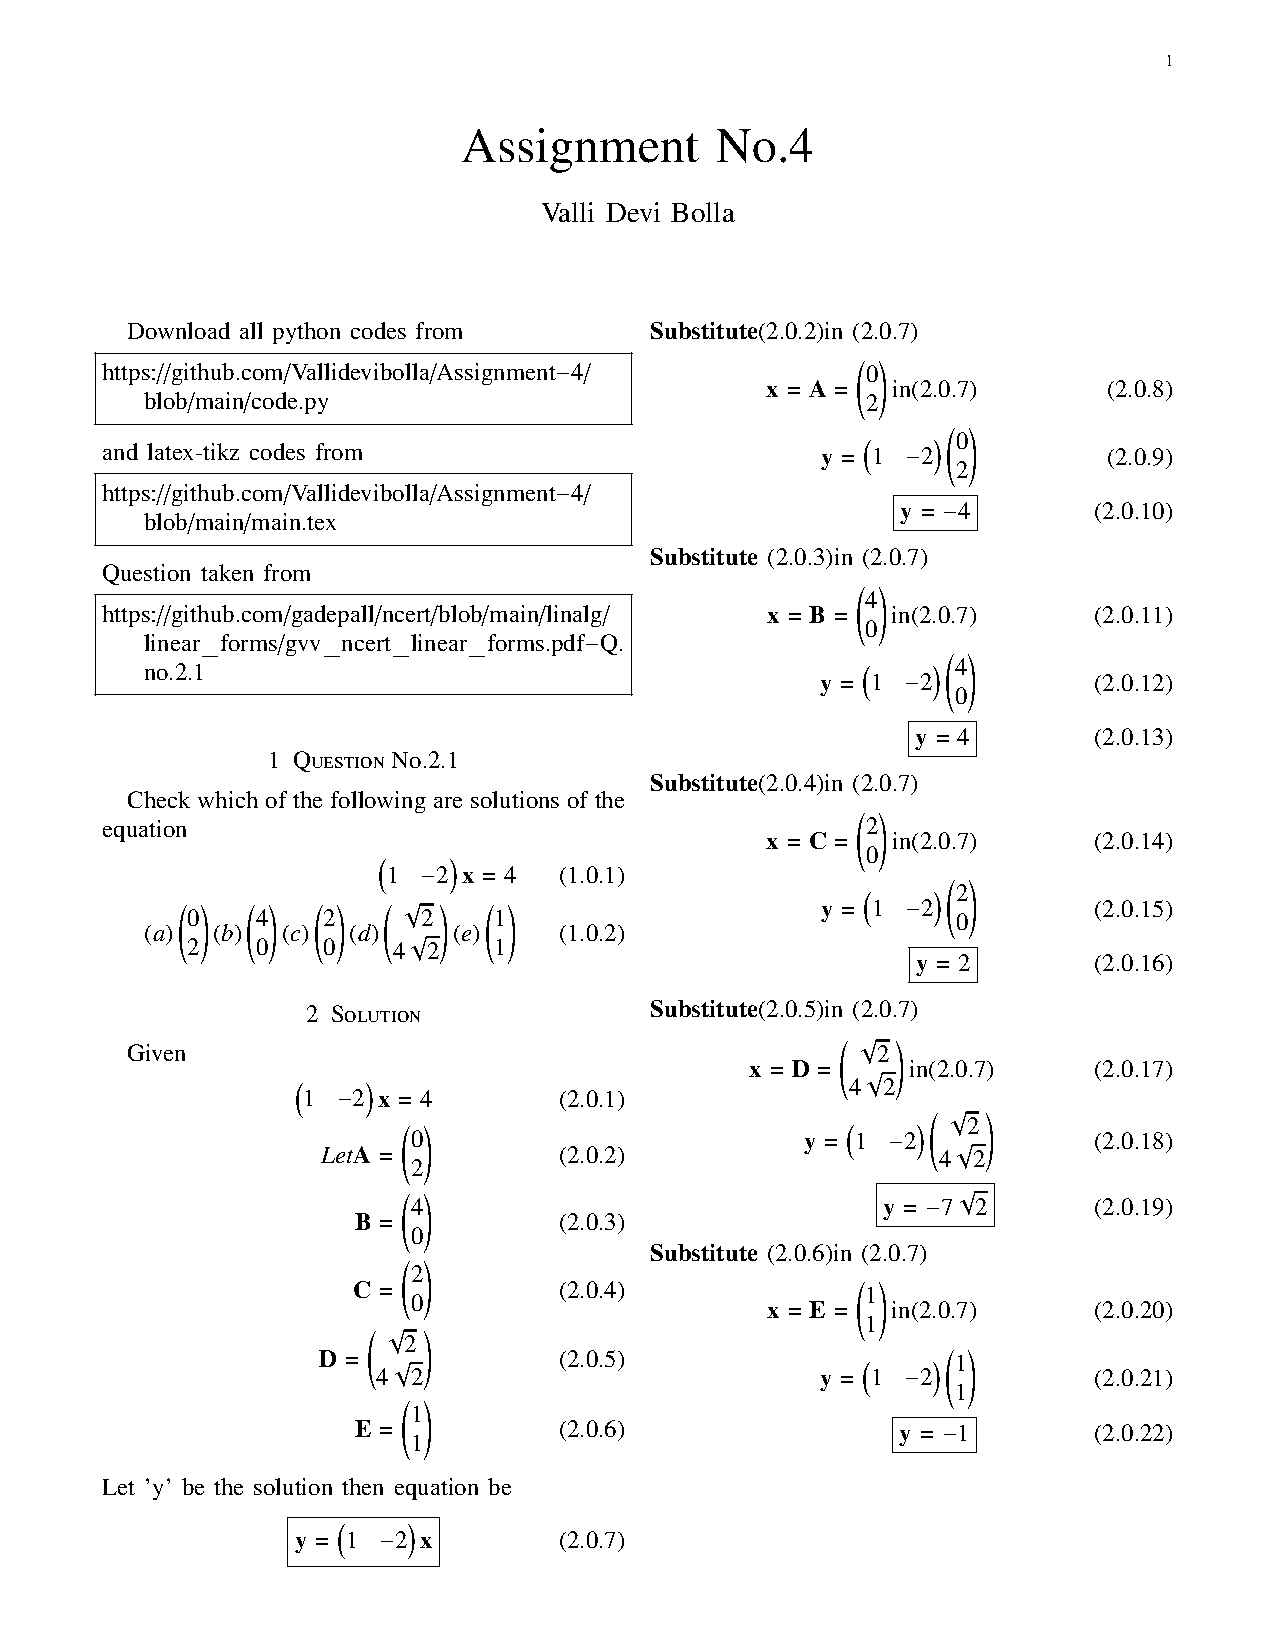
\includegraphics[width=\columnwidth]{solutions/aug/2/1/Assign_4 (7).pdf}
    \caption{Solution}
    \label{aug/2/1fig:Fig 2.1}
\end{figure}


